\documentclass[11pt]{article}

\usepackage{deauthor}
\usepackage{times,graphicx}

% user packages
\usepackage{todonotes}
\usepackage{pifont}
\newcommand{\cmark}{\ding{51}}
\newcommand{\xmark}{\ding{55}}
\usepackage{multirow}
\usepackage{booktabs}
\usepackage{graphicx}
\usepackage{subfig}
\usepackage{amsfonts}
\usepackage{amsmath}
\usepackage{amssymb}
\usepackage{booktabs}
\usepackage{pifont}
\newcommand{\ulnewnew}[1]{\underline{#1}}
\usepackage{makecell}
\usepackage{multirow}
\usepackage{multicol}
\newcommand{\mr}[3]{\multirow{#1}{#2}{#3}}
\newcommand{\mc}[3]{\multicolumn{#1}{#2}{#3}}
\renewcommand{\mathbf}[1]{\boldsymbol{#1}}
%\usepackage{enumitem}
\usepackage{wrapfig}
\def\modelname{HyCLID}
\def\figwidth{0.28}
\def\detailfigwidth{0.31}
\def\visualfigwidth{0.31}
\newcommand{\tabincell}[2]{\begin{tabular}{@{}#1@{}}#2\end{tabular}}


\title{Hypergraph Clustering Network for Interaction Data}

\author{Tianchi Yang$^{\dagger}$
\hspace{2em} Luhao Zhang$^{\ddagger}$
\hspace{2em} Cheng Yang$^{\dagger}$ \\
Chuan Shi$^{\dagger}$
\hspace{2em} Maodi Hu$^{\dagger}$
\hspace{2em} Tao Li$^{\dagger}$
\hspace{2em} Dong Wang$^{\dagger}$ \\
$^{\dagger}$ Beijing University of Posts and Telecommunications, Beijing, China \\
\texttt{\small\{yangtianchi,shichuan\}@bupt.edu.cn, albertyang33@gmail.com}\\
$^{\ddagger}$ Meituan, Beijing, China \\
\texttt{\small\{zhangluhao,litao19,wangdong07\}@meituan.com, Londeehu@gmail.com}}

% unnecessary commands
\usepackage{paralist}
\newcommand{\entity}{\mathcal{E}}
\newcommand{\relation}{\mathcal{R}}
\newcommand{\lang}{\mathcal{L}}
\newcommand{\model}{\mathcal{M}}
\newcommand{\term}{\mathcal{T}}
\newcommand{\kgnew}{\mathcal{KG}}

\begin{document}
\maketitle
\begin{abstract}
	With the rapid development of social media, the data generated from interaction, which is an action collaboratively done by several objects under a certain condition, have grown exponentially. It triggers an urgent need to cluster interaction data for implicit patterns benefiting downstream tasks. Although clustering methods have been extensively studied for a long time, they mainly focus on node/object clustering, which breaks the intrinsic collaborative associations among the involved objects and conditions, thus limiting clustering performance of interaction data. To tackle this issue, we propose a novel Hypergraph CLustering network for Interaction Data (\modelname), which not only clusters whole interactions rather than individual objects in interactions, but also exploits correlation among attributes of objects and conditions. Specifically, we first construct an attributed hypergraph to model interactions. Then, we propose a novel rethinking-based hypergraph neural network to learn the representation of interactions, which employs a novel attentive routing-based rethinking mechanism to capture the correlations among multiple object attributes and condition attributes. Furthermore, a novel adaptive mini-batch method is designed for the large scale of interaction data. Experimental results demonstrate the effectiveness of our methods for clustering the interactions and the practical value of the discovered interaction patterns.
\end{abstract}

\section{Introduction}  \label{sec:introduction}
% \vspace{-4pt}
With the rapid development of social media, the volume of interaction data\footnote{The term interaction data is similar to the term relational data, which focuses on the data that there are pair-wise relations \textit{between} objects, while we introduce the term interaction data in this paper for distinction to focus on the relations among multiple objects. } has grown exponentially to an overwhelming scale~\cite{kou_social_2016,yang_co-clustering_2022}.
Generally, an interaction is an action collaboratively done by several objects under a certain condition~\cite{yang_co-clustering_2022}. For example, as illustrated in Figure~\ref{fig:example}, ``a user ordered a cup of latte at Starbucks in the afternoon'' in food delivery systems, and ``two researchers collaborated to publish a paper in WSDM in 2022'' in academic networks, etc. In detail, Interaction 1 involves a condition about period and three objects including a user, a merchant and a product, each of which carries several attributes, which indicates the characteristic of interaction data is that the interaction involves multiple objects and the rich correlations among the attributes of objects and conditions.
As interaction data play an increasingly important role in daily life, analyzing them becomes a priority.

\begin{figure}%[!ht]
	\centering
	% \vspace{-5pt}
	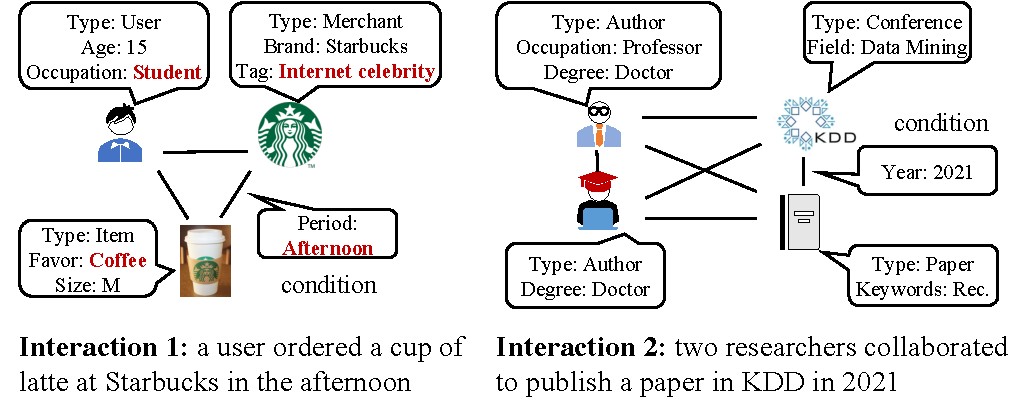
\includegraphics[width=0.70\linewidth]{submissions/HyCLID/figures/example.pdf}
	\caption{Examples of interactions from Meituan Waimai\protect\footnotemark[2] and academic networks. }
	\label{fig:example}
	% \vspace{-5pt}
\end{figure}
\footnotetext[2]{Meituan Waimai is a food delivery platform. https://waimai.meituan.com}

As a fundamental task in data mining, clustering on interaction data can discover the underlying patterns beneficial to downstream tasks. For instance, in the above example, the user preference can be found by clustering his interactions, enabling the platform to provide better recommendation services. Traditional clustering focuses on object features, such as K-means~\cite{hartigan_algorithm_1979,zhang_maximum_2021}, etc. Besides, graph-based clustering, which treats objects as nodes in a graph and leverages structural information of objects for clustering the objects, has also been widely explored, e.g., spectral clustering~\cite{ng2001spectral}. Recently, some researchers pay attention to attributed graph clustering, which jointly considers node attributes and graph structure~\cite{yang_effective_2021}. A noticeable trend is the wide adoption of deep learning in clustering~\cite{min_survey_2018}. For example, Graph Neural Network (GNN) based clustering methods~\cite{bo_structural_2020,wang_attributed_2019,song_deep_2021,yang_variational_2021} can effectively learn object representations for clustering via message passing mechanism. However, we argue that existing methods could not fully cope with the interaction data in the real world. Specifically, in interaction data, multiple objects as well as interaction conditions collaboratively form an indivisible semantic unit. Nonetheless, these methods focus on clustering individual nodes/objects, which breaks the intrinsic collaborative associations among the involved objects and conditions, thus limiting their ability to discover the underlying interaction patterns. Take Interaction 1 in Figure~\ref{fig:example} as an example, if we ignore the associations among user, merchant and product, one may discover a one-sided pattern that ``this user loves coffee''. This pattern will possibly lead to an inappropriate recommendation of high-end coffee to this student far beyond his consumption level.


Therefore, we propose to cluster interactions instead of objects, where each interaction is regarded as a basic unit to be clustered. Nevertheless, this is not a trivial task due to the following reasons:
(1) \textit{How to effectively model interaction data involving multiple objects? }
As mentioned before, an interaction is an indivisible semantic unit. Nevertheless, a majority of existing solutions employ graph structure to model the relations between objects, which will break the collaborative association among multiple objects into several pairwise sub-relations. Hence they are insufficient to model interaction data in the real world.
(2) \textit{How to capture the correlations among the attributes of objects and conditions? }
The occurrence of an interaction is mainly owing to the complex correlation among rich attributes of its involved objects and conditions. For instance, Interaction 1 in Figure~\ref{fig:example} is mainly derived by the correlation among ``student, Internet celebrity, coffee, afternoon'' (marked in red). Since this correlation is among multiple attributes,  capturing them is a combinatorial optimization problem. To avoid combinatorial explosion, some recent methods~\cite{song_autoint_2019,xu_disentangled_2021} adopt self-attentive layers to capture the pairwise correlations between two features, called second-order features. Then, the higher-order features can be approximated by stacking multiple self-attentive layers with residual connections.
However, the errors in the bottom layers will inevitably propagate to the following layers. Even worse, such error propagation will be enlarged as the number of layers increases, thus possibly leading to the omissions of some potential high-order features.
(3) \textit{How to handle the large scale of interaction data during clustering? }
The scale of interaction data in real applications is always large, thus requiring clustering in a batch fashion. Nonetheless, the data distributions of different batches are usually not the same, which probably causes data imbalance so that the clustering error may largely fluctuate or even increase~\cite{yan_deep_2015}.
Unfortunately, existing methods~\cite{xie_unsupervised_2016,wang_attributed_2019} cannot automatically make adaptive adjustments for different batches, thereby leading to sub-optimal clustering performance.

To tackle the aforementioned issues, we propose a novel Hypergraph CLustering network for Interaction Data (\modelname).
Specifically, to model interactions that involve multiple objects and conditions, we construct an attributed hypergraph for interactions. As the hyperedges can connect an arbitrary number of objects, we model each interaction as a hyperedge connecting several nodes that represent its involved objects. Then, we propose a novel rethinking-based hypergraph neural network to capture the complex correlations (high-order features) among object attributes and conditions for embedding the interactions (hyperedges). Besides, to avoid omissions of potential high-order features, we design a novel attentive routing-based rethinking mechanism to review the capturing process and correct the errors in the bottom layers. Finally, we propose an adaptive mini-batch clustering method based on the learned interaction representations to perform deep clustering on large-scale interaction data, which employs an adaptive batch standardization to remove the impact of different data distributions of different batches.
The main contributions are summarized as follows:

\begin{itemize} % [leftmargin=*]
	\item We propose a hypergraph clustering network for interaction data, namely \modelname. With interactions modeled as an attributed hypergraph, \modelname~designs a novel rethinking-based hypergraph neural network to learn the representation of interactions.
	
	\item Besides, we propose an adaptive mini-batch clustering method in the face of the large scale of the interaction data, which performs deep clustering in a mini-batch fashion based on the learned interaction representations.
	
	\item Experiments show that \modelname~significantly outperforms state-of-the-art methods across public and industrial datasets for clustering interactions. Furthermore, experiments on recommendation demonstrate the practical value of the cluster patterns discovered by our method in industrial applications.
\end{itemize}


\section{Related Work}
% \vspace{-4pt}
In this section, we first introduce the related clustering methods, and then discuss the hypergraph approaches for interaction data.

Clustering, as one of the fundamental tasks of data mining, is widely used for interaction data analysis.
Traditional clustering studies are feature-based. They can target a certain type of interacting objects, and encode them as vectors based on their features~\cite{hinton_reducing_2006} followed by traditional clustering methods such as K-means~\cite{hartigan_algorithm_1979}.
Besides, graph-based clustering is also a representative kind of clustering method, which treats objects as nodes in a graph and leverages structural information of objects for clustering the objects, e.g., spectral clustering~\cite{ng2001spectral}. Recently, attributed graph clustering has attracted a mass of attention, which further considers the attributes of nodes~\cite{yang_effective_2021}. A noticeable trend is the wide adoption of deep learning in clustering~\cite{min_survey_2018}. For example, Graph Neural Network (GNN)~\cite{kipf_semi_supervised_2017,kipf_variational_2016} based clustering methods can effectively learn representations based on the graph structure and node attributes for clustering~\cite{bo_structural_2020,wang_attributed_2019,fan_one2multi_2020,song_deep_2021,yang_variational_2021}.
However, modeling the interaction data using the graph structure, which can only model the pairwise relations, will inevitably lose some information since an interaction usually involves more than two objects~\cite{yang2020hypergraph}.


Hypergraphs, as generalizations of graphs, can model complex and extensive information and be more suitable for interaction data~\cite{zhang_hyper_sagnn_2020,yadati_hypergcn_2019,tran_directed_2020,hu_adaptive_2021}.
How to develop hypergraph structure based solutions for interaction data attracts increasing attention. \cite{zhou_learning_2006} puts forward the concept of learning with hypergraphs, which can be used in clustering, classification, and embedding and achieves performance beyond the ordinary graphs. Hypergraph neural networks (HGNN) proposed in~\cite{feng_hypergraph_2019}, which are similar to the GCNs in graphs~\cite{kipf_semi_supervised_2017}, extend the convolution operation to the process of hypergraph learning. \cite{zhu_adaptive_2017} proposes an unsupervised method to conduct both subspace learning and feature selection, but its complex optimization details do not make it perform better than the above graph methods for clustering tasks. A recent study thereby proposes an end-to-end clustering method based on hypergraph neural network~\cite{hu_adaptive_2021}.
However, these methods only target the individual node/object, which breaks the intrinsic collaborative associations among the involved objects and conditions. The related works for clustering the interactions still are little exploration.



\section{Methodology}    \label{sec:model}
% \vspace{-4pt}
\begin{figure*}%[!ht]
	\centering
	% \vspace{-5pt}
	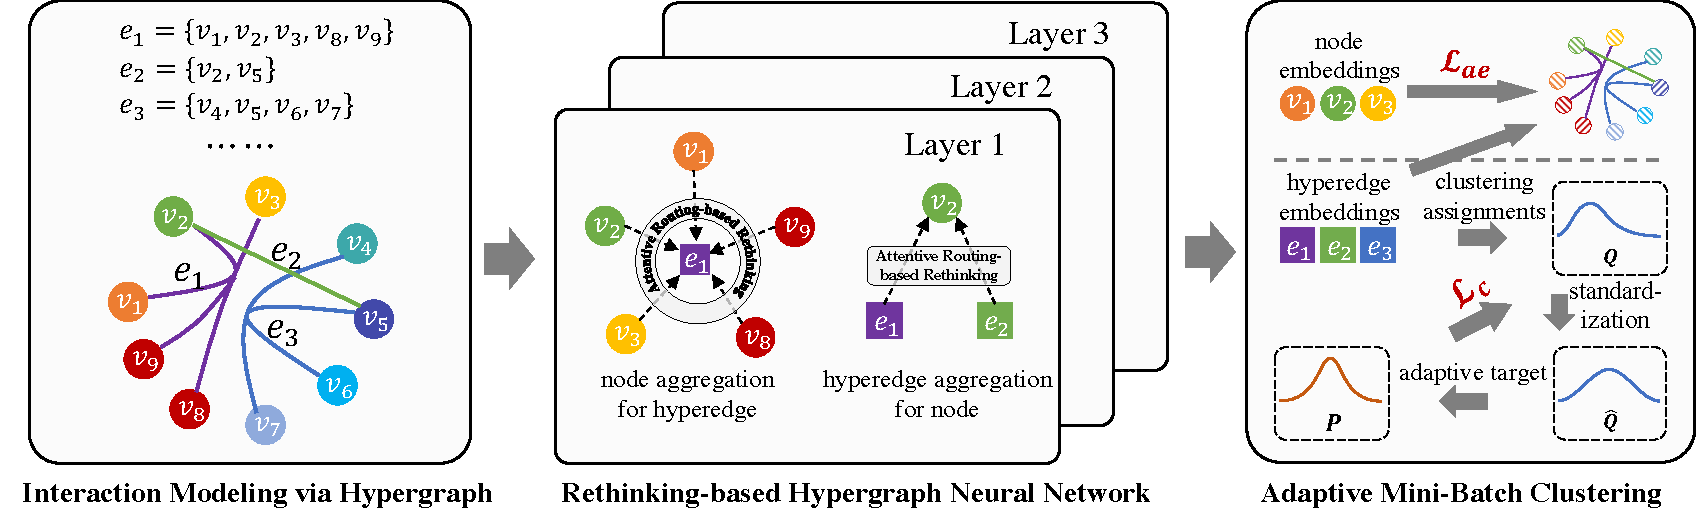
\includegraphics[width=0.93\linewidth]{submissions/HyCLID/figures/model}
	\caption{Illustration of \modelname~(object attributes and interaction conditions are omitted for easy to understand). }
	\label{fig:model}
	% \vspace{-15pt}
\end{figure*}
%\subsection{Overview}   \label{mod:overview}
First of all, we present an overview of the proposed \modelname.
The basic idea is that, as illustrated in Figure \ref{fig:model}, with modeling interactions via attributed hypergraph, we propose a novel rethinking-based hypergraph neural network to learn the representations of interactions for clustering. Specifically, to model the interactions that involve multiple objects and conditions, we construct an attributed hypergraph, where each interaction is modeled as a hyperedge connecting several nodes that represent its involved objects. Besides, the attributes of objects and conditions are introduced as node features and hyperedge features, respectively. Then, a novel rethinking-based hypergraph neural network is proposed to aggregate node and hyperedge features to obtain interaction and object representations. During feature aggregation, we design a novel attentive routing-based rethinking mechanism, which can capture high-order features and then rethink to check for omissions and errors. Finally, in the face of the large scale of the interaction data, we develop an adaptive mini-batched clustering method to cluster in a mini-batch fashion based on the learned interaction representations. Moreover, it employs an adaptive batch standardization to remove the impact of different data distributions of different batches.


\subsection{Interaction Modeling via Hypergraph}   \label{mod:construction}
%In this subsection, we detail the modeling of interactions via attributed hypergraph.

As mentioned above, an interaction usually involves multiple attributed objects and the corresponding interaction conditions such as temporal-spatial contexts, etc. We formalize the \textit{interactions} as follows.

\begin{definition}   \label{def:interaction}
	\textbf{Interaction. }
	An interaction is an action collaboratively done by several objects under a certain condition. Formally,
	given the set of objects $ \mathcal{V} $, object attributes $ A^\mathcal{V} $, and interaction conditions $ A^\mathcal{E} $, an interaction is defined as $ e = <\mathcal{V}_e, A^\mathcal{V}_e, A^\mathcal{E}_e> $, including all involved objects $ \mathcal{V}_e = \{ v_1, \cdots, v_{n_e} | v_i \in \mathcal{V} \} $ with their attributes $ A^\mathcal{V}_e = \{ a_1, \cdots, a_{n_e} | a_i \subset A^\mathcal{V} \} $, and interaction conditions $ A^\mathcal{E}_e \subset A^\mathcal{E} $.
\end{definition}

Take Interaction 1 in Figure~\ref{fig:example} as an example, ``a fifteen-year-old student ordered a middle-size latte at the Internet celebrity store Starbucks in the afternoon''. In this example, the interaction \textit{order} involves the objects including a user (with occupation attribute \textit{student} and age attribute \textit{fifteen}), a merchant (with attribute \textit{Starbucks} and \textit{Internet celebrity}) and an item \textit{coffee} (with attribute \textit{latte} and \textit{middle-size}). Besides, this interaction has a condition \textit{afternoon}.
In order to avoid the association breaking in traditional graph modeling, which splits the collaborative association among multiple objects into several pairwise sub-relations, we model the interactions as an attributed hypergraph.

In detail, each of the interactions is modeled as a hyperedge connecting several nodes that represent its involved objects.
Moreover, object attributes are the features of corresponding nodes, and condition attributes are the features of the hyperedges.
For example, as illustrated in left of Figure~\ref{fig:model}, for an interaction $ e_1 $ involving 5 objects $ v_1, v_2, v_3, v_8, v_9 $, we build a hyperedge to connect them. Besides, we attach their object attributes $ a_i (i=1,2,3,8,9) $ to the node features. Then the condition attributes $ \breve{A}_{e_1}^\mathcal{E} $, such as temporal-spatial contexts, are attached to the hyperedge features, since they should be seen as the attributes of interactions rather than any object. Therefore, such a hyperedge and its connecting nodes together with their features can represent an instance of interactions.
The constructed attributed hypergraph is formalized as follows.
\begin{definition}   \label{def:hypergraph}
	\textbf{Attributed Hypergraph for Interactions. }
	The hypergraph for interactions is an attributed hypergraph $\mathcal{G}=$ $(\mathcal{V}, \mathcal{E}, \boldsymbol{X}_V, \boldsymbol{X}_E)$, where the node set $\mathcal{V}$ represents the set of all involved objects, the hyperedge set $\mathcal{E}$ represents all the interactions, $\boldsymbol{X}_V$ and $\boldsymbol{X}_E$ represent the feature matrices of nodes and hyperedges, respectively.
\end{definition}
The $i$-th row of $\boldsymbol{X}_V \in \mathbb{R}^{|\mathcal{V}| \times F_V}$ represents the feature indicators to the  attributes $ a_i \subset A^\mathcal{V} $ of object $ v_i \in \mathcal{V} $. Similarly, the $j$-th row of $\boldsymbol{X}_E \in \mathbb{R}^{|\mathcal{E}| \times F_E}$ represents the feature indicators to the condition attributes $ A^\mathcal{E}_{e_j} \subset A^\mathcal{E} $ of interaction $ e_j \in \mathcal{E} $. $F_V$ and $F_E$ are the max value across the attribute number of each object and condition, respectively.

Based on the above modeling, the clustering task of interactions in this paper can be formalized as the clustering on hyperedges $\mathcal{E}$ in the constructed attributed hypergraph, which is different from other clustering methods that mainly concern about clustering of objects $\mathcal{V}$ in interactions~\cite{hu_adaptive_2021}.


\subsection{Rethinking-based Hypergraph Neural Network}    \label{mod:hgnn}
% \vspace{-4pt}
To learn the representation of interactions, we propose a novel rethinking-based hypergraph neural network, where an attentive routing-based rethinking mechanism is designed to capture high-order features and avoid omissions. It can automatically identify the correlations of features and form some meaningful combinations of high-order features. Then, it rethinks the identification process several times to prevent omissions and correct errors. Consequently, the network can learn effective representation of interactions.

\subsubsection{Input Layer. }
In order to facilitate capturing high-order features, following~\cite{song_autoint_2019}, we initial the representations of each feature from hyperedges or nodes as vectors, thus the representations of hyperedges and nodes are formed as feature matrices. Formally, the initial $d$-dimensional representations of hyperedge $ e_i \in \mathcal{E} $ and node $ n_j \in \mathcal{N}$ are
$
\boldsymbol e_i^{(0)} \in \mathbb{R}^{F_E \times d}  $ and $  \boldsymbol v_j^{(0)} \in \mathbb{R}^{F_V \times d} ,
$
where each row of the feature matrix denotes a specific attribute of the node/hyperedge.

\subsubsection{Layer-wise Aggregation. }
For the hypergraph $\mathcal{G}$, the incidence matrix is defined as $\boldsymbol{H} \in \mathbb{R}^{|\mathcal{V}| \times|\mathcal{E}|}$ with entries $h(v, e)=1$ if $v \in e$ and 0 otherwise. Denote the diagonal matrices of the edge degrees, the node degrees and the pre-defined weights of hyperedges (default is 1) as $ \boldsymbol{D}_{e} $, $ \boldsymbol{D}_{v} $ and $ \boldsymbol{W} $, respectively. The spectral hypergraph convolution for node embedding~\cite{feng_hypergraph_2019,hu_adaptive_2021} is formulated as
\begin{align}
	\boldsymbol{Y}=\boldsymbol{D}_{v}^{-1/2} \boldsymbol{H} \boldsymbol{W} \boldsymbol{D}_{e}^{-1} \boldsymbol{H}^{\top} \boldsymbol{D}_{v}^{-1/2} \boldsymbol{X}_V \boldsymbol{\Theta},
\end{align}
where $ \boldsymbol{\Theta} $ is the trainable filter parameters and $ \boldsymbol{X}_V $ is the input node embeddings. It can be seen that in this hypergraph convolution formula, neither can the features of the hyperedge be exploited, nor can the representation of the hyperedges (interactions) be obtained.

To solve these problems, we analyze this formula intuitively and find that this form can be also understood as the following information flow: The node embeddings are first aggregated into hyperedge embeddings by multiplying matrix $ \boldsymbol{H}^\top $. Then the hyperedge information is passed back to the nodes, achieved by multiplying $ \boldsymbol{H} $. We can formalize these two information aggregation processes as a two-stage aggregation rule from layer $l$ to layer $l+1$ as follows.
\begin{align}
	\boldsymbol e^{(l+1)}_i &= \text{aggr}(\boldsymbol e^{(l)}_i, \{\boldsymbol v^{(l)}_j \, | \, v_j \in e_i\})  \label{eq:e_aggr}, \\
	\boldsymbol v^{(l+1)}_j &= \text{aggr}(\boldsymbol v^{(l)}_j, \{\boldsymbol e^{(l+1)}_i \, | \, v_j \in e_i\})  .
\end{align}
For the aggregation function $ \text{aggr}(\cdot) $, we first concatenate all its inputs into an whole feature matrix $ X = \text{concat}(\boldsymbol e^{(l)}_i, \{ \boldsymbol v^{(l)}_j | v_j \in e_i \}) $ or $ X = \text{concat}(\boldsymbol v^{(l)}_j, \{\boldsymbol e^{(l+1)}_i | \\ v_j \in e_i\})$, then we propose the following module to capture the high-order features based on $ X $ before obtaining the node/hyperedge embeddings.
Please note that the size of $X$ is not fixed. The number of its rows depends on the number and size of the concatenated feature matrices of hyperedges and nodes. For example, the size of the whole feature matrix for Eq.~\ref{eq:e_aggr} is $ (F_E + |e_i| \cdot F_V) \times d $.
Denoting the calculation of this module as function ARR$(\cdot)$ for short, the aggregation function can be formalized as $ \text{aggr}(\cdot) = \text{ARR}(\text{concat}(\cdot))$.


\subsubsection{Attentive Routing-based Rethinking Mechanism } \label{mod:routing}
As introduced before, the interactions often arise from the intrinsic correlations among several related attributes. Motivated by previous studies~\cite{song_autoint_2019,xu_disentangled_2021}, the correlations among $p$ attributes are formalized as a $p$-order features. As shown in Figure~\ref{fig:routing}, we adopt the framework of multiple self-attentive layers to capture high-order features. Furthermore, in order to prevent omissions of potential high-order features, we need to review the capturing process to check for omissions and errors. Consequently, we introduce a routing mechanism and modify the self-attentive layers to rethink and readjust the captured high-order features. The details are introduced as follows.

% \begin{figure}%[!ht]
%  \centering
%  \includegraphics[width=0.45\linewidth]{figures/routing.pdf}
%  \caption{Illustration of the attentive routing-based rethinking mechanism. }
%  \label{fig:routing}
% \end{figure}
\setlength{\columnsep}{10pt}%
\begin{wrapfigure}{r}{0.45\linewidth}
	\centering
	% \vspace{-20pt}
	\includegraphics[width=\linewidth]{submissions/HyCLID/figures/routing.pdf}
	\caption{Illustration of the attentive routing-based rethinking mechanism. }
	% \vspace{-20pt}
	\label{fig:routing}
\end{wrapfigure}
Following~\cite{song_autoint_2019,xu_disentangled_2021}, we adopt the framework of self-attention to learn high-order features due to its superiority for saving computational and storage. However, it needs further improvement to support rethinking. Specifically, we introduce a rethinking vector $ \hat{z} $, the attention score between feature $ x_m $ and $ x_k $, i.e., the $m$-th and $k$-th rows of the input feature matrix $X$, is calculated as,
\begin{align}
	\varphi(\hat{z}; x_m, x_k) = \text{sum} \left( \hat{z} \odot W_{\text{Q}} x_m \odot W_{\text{K}} x_k \right),  \label{eq:phi}
\end{align}
where $ \odot $ represents element-wise product, i.e., Hadamard product. $ W_{\text{Q}} $ and $ W_{\text{K}} $ denote the transformations for Query vector and Key vector in attention. Then the group of second-order features related to feature $ x_m $ can be combined together through the framework of self-attention as follows.
\begin{align}
	& \alpha_{m, k} = {\exp \left(\varphi(\hat{z}; x_m, x_k)\right)} \ /\  {\sum\nolimits_{j=1} \exp \left(\varphi(\hat{z}; x_m, x_j)\right)}, \label{eq:alpha} \\
	& x_m^{(2)} = x_m + \sum\nolimits_{k=1} \alpha_{m, k}(W_{\text{V}} e_{k}) ,  \label{eq:highorder}
\end{align}
where $ W_{\text{V}} $ denotes the transformation for Value vector in attention. Next, a higher-order feature $ x_m^{(p)} $ related to $ x_m $ can be captured by stacking $ p-1 $ layers of such self-attention with residue connections. Eventually, the final combination $ \hat{z}^{(1)} $ of feature of order $ p $ can be obtained by attentive fusion of $x_m^{(p)}, m=1,2,\cdots$,
\begin{align}
	\hat{z}^{(1)} &= \sum\nolimits_m \text{SoftMax} \left( (\hat{z} \odot \boldsymbol x_m^{(p)})^\top \cdot \boldsymbol a \right) \cdot \boldsymbol x_m^{(p)} \ ,   \label{eq:update}
\end{align}
where $ \boldsymbol a $ is the vector of attention parameters.


Furthermore, to prevent omissions of potential high-order features, we introduce a routing mechanism to rethink and readjust the above capturing process. Specifically, we update the rethinking vector by the new obtained $ \hat{z}^{(1)} $, and repeat the above procedure  several times until routing-by-agreement, which is called attentive routing-based rethinking mechanism. Therefore, each repetition of the above process, i.e., each iteration of the routing mechanism, refines the captured high-level features. Initially, let $\hat{z} = \text{mean}_m (W_{\text{V}} x_m)$.

The output high-order feature after repeating $r$ times is denoted as $ \hat{z}^{(r)} $, which is the output vector of this module. Formally, given an input feature matrix $X$, we have $ \text{ARR}(X) = \hat{z}^{(r)} $.
Then, the Eq.~\eqref{eq:e_aggr} can be rewritten by $ \boldsymbol e^{(l+1)}_i = \text{ARR}(X) $, where $ X $ is obtained by concatenating the embedding matrices of a target hyperedge and its connecting nodes.


\subsubsection{Interaction \& Object Embedding. }
Since each layer of propagation represents a specific order\footnote{Please note that the order of relations is the path length between neighbors and the target node, while the order of features is the number of features combined into high-order feature.} of relations, we sum the embeddings from each layer as the final representation both for hyperedges (interactions) and nodes (objects). Formally, we have
$
\boldsymbol e_i = \sum\nolimits_l^L \boldsymbol e^{(l)}_i $ and $ \boldsymbol v_j = \sum\nolimits_l^L \boldsymbol v^{(l)}_j ,
$
where $L$ denotes the number of aggregation layers.


\subsection{Adaptive Mini-batch Clustering}    \label{mod:batch}
% \vspace{-4pt}
For clustering in a mini-batch fashion, the different data distributions of batches may lead to clustering errors~\cite{yan_deep_2015}, thus making clustering difficult to discover the implicit patterns of interaction data. Therefore, enlightened by existing deep clustering methods~\cite{xie_unsupervised_2016}, we propose an adaptive mini-batch clustering method, which first removes the impact of different data distributions via an adaptive batch standardization and then performs deep clustering on interactions.

Specifically, after the above modules, we have obtained the representations of interactions. Enlightened by Clustering Assignment Hardening~\cite{xie_unsupervised_2016}, we take Student's $t$-distribution as a kernel to measure the similarity between points and centroids.
Then the soft assignment matrix $Q$ is formulated as follows:
\begin{align}
	q_{i j}=\frac{(1+\|z_{i}-\mu_{j}\|^{2} / \nu)^{-\frac{\nu+1}{2}}}{\sum_{j^{\prime}}(1+\|z_{i}-\mu_{j^{\prime}}\|^{2} / \nu)^{-\frac{\nu+1}{2}}} ,
\end{align}
where $z_{i}$ is the embedding of the $i^{th}$ interaction, $\mu_{j}$ is the $j^{th}$ cluster centroid, and $\nu$ is the degrees of freedom of the Student’s t-distribution, e.g. $\nu=1$.

Due to the randomness of batch generating process, the assignment distribution $Q$ can be very unstable. It severely limits the robustness of clustering, which in turn brings difficulties to discovering patterns in interaction data. To tackle this issue, we first square the $Q$ distribution to speed up training and then batch standardize it to obtain $\hat{Q}$, which removes the influence of batch quality on the clustering performance. Formally,
\begin{align}
	& \widehat{q}_{iu}  = ({q^2_{iu}-\mu_{u}}) \, / \, ({\sqrt{\sigma_{u}^{2}+\epsilon}}) \, , \\
	\text{where }\ \,  \mu_{u}  = \frac{1}{m} &\sum\nolimits_{i} q^2_{iu} \ \, \text{ and } \ \,
	\sigma_{u}^{2}  = \frac{1}{m} \sum\nolimits_{i}\left(q^2_{iu}-\mu_{u}\right)^{2} .
\end{align}
Note that this standardization operation makes $\hat{Q}$ appear negative numbers. It means that we can just erase the low-probability cluster assignment via ReLU function, which contributes to to reduce the difficulty of clustering training and improve performance. Furthermore, we introduce two batch adaptive trainable parameters $ \gamma, \beta $ to enhance its adaptive ability as follows.
\begin{align}
	p_{iu} & = \frac{\text{ReLU}( \gamma_{u}  \widehat{q}_{iu} + \beta_{u} )}{\sum\nolimits_{s} \text{ReLU}( \gamma_{s}  \widehat{q}_{is} + \beta_{s} )} \ , \qquad s.t. \sum\nolimits_u \gamma_u = 1  ,
\end{align}
where $\gamma $ represents the relative stability between different clusters (small value means that the samples of one cluster are prone to be modified to another cluster during training), and $\beta$ defines the aforementioned low-probability cluster assignment. Consequently, the adaptive target distribution $ P = [p_{i u}] $ forces assignments to have stricter probabilities (closer to 0 or 1). Meanwhile, we not only preserve the stability of the $Q$ distribution by $\hat{Q}$, but also increase its adaptive capacity. Finally, KL-divergence is applied to let the raw assignments $Q$ approach the target distribution $P$.
% \begin{align}
%     \mathcal{L}_{c}=\mathrm{KL}(P \| Q)=\sum_{i} \sum_{j} p_{i j} \log \frac{p_{i j}}{q_{i j}} ,   \label{eq:klpq}
% \end{align}
which can be minimized for the aforementioned $Q$ and $P$ via neural network training. It emphasizes data points assigned with batch-adaptive high confidence.

\subsection{Model Training}
% \vspace{-4pt}
We apply an auto-encoder structure for self-supervised training of our \modelname. Specifically, we reconstruct the incidence matrix $ H $ of the constructed hypergraph for interactions with a contrastive loss:
\begin{align}
	\mathcal{L}_{ae} = \frac{1}{2} \sum_{i, j} y_{ij} d_{ij}^2 + (1-y_{ij}) \text{max}(0, m - d_{ij})^2  , \quad
	\text{where } \ \, {d}_{ij} = \| \boldsymbol e_i - \boldsymbol v_j \|  .
\end{align}
$ y_{ij} $ denotes the existence of a relationship between hyperedge $ i $ and node $ j $, and $ m $ is the margin hyper-parameter, e.g., $ m = 1 $.

Finally, we jointly optimize the auto-encoder structure and deep clustering so that the total objective function is defined as
$
\mathcal{L} = \mathcal{L}_{c} + \gamma \mathcal L_{ae},
$
where $ \gamma \geqslant 0 $ is a coefficient that controls the balance in between.


\section{Experiments}       \label{sec:experiment}

\subsection{Experimental Setup}		\label{exp:setup}
% \vspace{-4pt}
\subsubsection{Datasets}
\begin{table*}% []    

\caption{Statistics of datasets. }
\centering
\resizebox*{0.98\linewidth}{!}{
\begin{tabular}{l rl rl rl cccc}
\toprule
Dataset & \multicolumn{6}{c}{\# Nodes}                           & \# Hyperedges & \# Attributes & \# Categories & Graph Density    \\
\cmidrule(lr){1-11}
ACM     & Paper & 4,025   & Author   & 7,167  & Field  & 60      & 4,025         & 1,902         & 3             & $ \sim 10^{-4} $ \\
IMDB    & Movie & 4,661   & Director & 5,841  & Actor  & 2,270   & 4,661         & 1,256         & 3             & $ \sim 10^{-4} $ \\
MT-S    & User  & 19,623  & POI      & 6,489  & Item   & 17,564  & 20,000        & 901           & 5             & $ \sim 10^{-5} $ \\
MT-L    & User  & 991,914 & POI      & 17,120 & Item   & 389,292 & 2,000,000     & 901           & 5             & $ \sim 10^{-6} $ \\
\bottomrule
\end{tabular}
}
\label{tab:statistics}
\end{table*}

Our proposed \modelname~is evaluated on the following four datasets, and the statistics of these datasets are shown in Table~\ref{tab:statistics}.

\begin{itemize} %[leftmargin=*]
	\item \textbf{ACM. }
	The ACM dataset\footnote{https://data.dgl.ai/dataset/ACM.mat} contains three types of nodes: paper, author and field. We treat a publishing as an interaction, and hence build a hypergraph where each hyperedge connects a paper and all its corresponding authors and fields. Considering there are no labels on the hyperedges, we treat the category of the published paper as the clustering ground truth since each paper has a one-to-one correspondence to a hyperedge.
	
	\item \textbf{IMDB. }
	The IMDB dataset~\cite{yun_graph_2019} contains three types of nodes: movie, actors and directors. Similarly, we treat each movie as an interaction and construct a hypergraph where each hyperedge connects a movie, its actors and directors. The category of the movie is regarded as the clustering ground truth.
	
	\item \textbf{MT-L} and \textbf{MT-S. }
	We also build two real-world datasets from the food delivery industry, i.e., Meituan Waimai platform. % \footnote{https://waimai.meituan.com/}.
	One contains millions of orders of user purchases of foods in Beijing District within 30 days, denoting as MT-L. Each purchase order is treated as an interaction and is tagged with one of 5 purchase scenes. We construct an attributed hypergraph where each hyperedge represents an order, connecting a user node, a restaurant node and several item nodes. The features of nodes are their attributes (e.g., user profiles for user node), while the features of hyperedges (orders) are the interaction conditions, i.e., temporal-spatial contexts, since these attributes do not belong to a single node.
	Most baseline methods cannot support data of such scale, so we extracted a smaller dataset from it, denoted as MT-S.
\end{itemize}

\subsubsection{Evaluation Metrics}
Following~\cite{hu_adaptive_2021}, we adopt three popular metrics to assess the quality of the clustering results: clustering accuracy (ACC), normalized mutual information (NMI) and adjusted Rand index (ARI). For all the experiments, we repeat them 10 times and report the averaged results and standard deviations.

\subsubsection{Baselines}
We compare our proposed method \modelname~with the following three groups of methods.
% three groups of methods: traditional approaches, which only consider attributes or only structures; attributed graph-based methods, which are improved for end-to-end graph clustering; hypergraph-based methods, which employ hypergraph to model interactions.
{Traditional Methods: }
\textit{K-means}~\cite{hartigan_algorithm_1979}, \textit{node2vec}~\cite{grover_node2vec_2016} and \textit{HERec}~\cite{shi2018heterogeneous}.
{Attributed Graph-based Methods: }
\textit{SDCN}~\cite{bo_structural_2020}, \textit{HAN}~\cite{wang_heterogeneous_2019}, \textit{HGT}~\cite{hu_heterogeneous_2020} and \textit{AdaGAE}~\cite{li_adaptive_2021}.
{Hypergraph-based Methods: }
\textit{HGNN}~\cite{feng_hypergraph_2019} and \textit{AHGAE}~\cite{hu_adaptive_2021}.
%
%\begin{itemize}  [leftmargin=*]
%\item \textbf{Traditional Methods: }
%	\textit{K-means}~\cite{hartigan_algorithm_1979}: It is based on the multi-hot features over the whole attribute vocabulary.
%    \textit{node2vec}~\cite{grover_node2vec_2016}: It performs random walk followed by a Skip-Gram model for node embeddings. We apply K-means on these learned node embeddings.
%    \textit{HERec}~\cite{shi2018heterogeneous}: It is a heterogeneous graph embedding method which designs a type constraint random walk followed by skip-gram.
%
%\item \textbf{Attributed Graph-based Methods: }
%	\textit{SDCN}~\cite{bo_structural_2020}: It is a deep graph clustering model that combines the strengths of both attributes by autoencoder and structures by GCN.
%	\textit{HAN}~\cite{wang_heterogeneous_2019}: It is a heterogeneous graph neural network equipped with a node-level and a semantic-level attentions.
%	\textit{HGT}~\cite{hu_heterogeneous_2020}: It is a SOTA heterogeneous graph embedding model that incorporates the types of nodes and edges into the propagation step.
%	\textit{AdaGAE}~\cite{li_adaptive_2021}: It is a SOTA graph-based clustering method for general clustering with an adaptive graph auto-encoder. We adjusted it slightly based on our constructed graphs.
%
%\item \textbf{Hypergraph-based Methods: }
%	\textit{HGNN}~\cite{feng_hypergraph_2019}: It is a hypergraph spectral convolution network framework. We split its convolution into 2-stage for explicit hyperedge representation.
%	\textit{AHGAE}~\cite{hu_adaptive_2021}: It is a SOTA auto-encoder-based hypergraph method for relational data clustering. We similarly modify it like HGNN for explicit hyperedge representation.
%\end{itemize}
%
Note that for the methods considering graph structure, for ACM and IMDB datasets, we directly use the widely applied graph structure~\cite{hu_heterogeneous_2020}. For the MT-S dataset, we transfer the hypergraph into a graph, i.e., we introduce a summary node to replace each of hyperedges and link the summary nodes with the corresponding nodes that are originally connected by hyperedges.
For metapath-based methods, i.e., HERec and HAN, we select all the possible symmetric length-2 meta-paths.


\subsubsection{Implementation Detail}
We implement the proposed method based on Tensorflow\footnote{https://www.tensorflow.org/}. For our method, we set the dimension of attribute embeddings as $ d=64 $ for the public datasets ACM and IMDB for fair comparison and $ d=16 $ for MT-S/L for saving memory. For simplicity, we set the number of aggregation layers $L = 1$, the layer number of rethinking-based self-attention $p = 1$ and the rethinking iterations $r=2$. For all baselines, we set their hidden dimensions as 64 and set the number of layers as their suggested value (usually equal to 2). For model training, we simply set $ \gamma = 1 $, and apply Adam~\cite{kingma_adam_2015} to optimize with the learning rate as 0.005 for ACM and IMDB and 0.001 for MT-S/L. The batch size is set 2048. All the experiments are performed in NVIDIA Tesla P40 Cluster. To facilitate related research, we will release our implementation to the public once the paper gets accepted.


\subsection{Analysis of Clustering Results}
% \vspace{-8pt}
% 大表格
\begin{table*}%[!ht]
\caption{Clustering results on datasets ACM, IMDB and MT-S (mean$\pm$std in percent). The best and second best results are bold and underlined, respectively. Symbol ``-'' represents unavailable results due to out-of-memory. }
\centering
% \vspace{-4pt}
\resizebox*{0.99\linewidth}{!}{
\begin{tabular}{l|ccc|ccc|ccc}
\toprule
\multirow{2}{*}{Method} &
  \multicolumn{3}{c|}{ACM} &
  \multicolumn{3}{c|}{IMDB} &
  \multicolumn{3}{c}{MT-S} \\
\cmidrule(lr){2-4} \cmidrule(lr){5-7} \cmidrule(lr){8-10}
 &
  ACC & NMI & ARI & 
  ACC & NMI & ARI & 
  ACC & NMI & ARI \\
\cmidrule(lr){1-10} 
K-means &
  63.59 $\pm$ 0.27 &
  36.89 $\pm$ 0.37 &
  28.91 $\pm$ 0.42 &
  37.01 $\pm$ 0.10 &
  0.88 $\pm$ 0.06 &
  1.43 $\pm$ 0.05 &
  54.95 $\pm$ 8.08 &
  56.36 $\pm$ 6.69 &
  50.08 $\pm$ 7.83 \\
node2vec &
  65.25 $\pm$ 0.33 &
  38.49 $\pm$ 0.12 &
  31.23 $\pm$ 0.88 &
  47.87 $\pm$ 0.33 &
  {5.55 $\pm$ 0.53} &
  \underline{5.89 $\pm$ 0.64} &
  45.09 $\pm$ 6.70 &
  23.19 $\pm$ 5.60 &
  18.65 $\pm$ 7.78 \\
HERec &
  51.41 $\pm$ 1.82 &
  20.05 $\pm$ 1.37 &
  20.82 $\pm$ 1.50 &
  46.45 $\pm$ 0.62 &
  5.32 $\pm$ 0.79 &
  5.68 $\pm$ 0.69 &
  39.76 $\pm$ 9.72 &
  20.57 $\pm$ 2.04 &
  18.32 $\pm$ 3.11 \\
\cmidrule(lr){1-10} 
SDCN &
  67.79 $\pm$ 0.87 &
  41.77 $\pm$ 0.80 &
  37.69 $\pm$ 0.60 &
  43.87 $\pm$ 0.35 &
  3.37 $\pm$ 0.19 &
  2.77 $\pm$ 0.21 &
  73.56 $\pm$ 9.27 &
  66.34 $\pm$ 8.02 &
  62.80 $\pm$ 7.83 \\
HAN &
  69.33 $\pm$ 0.38 &
  44.17 $\pm$ 0.58 &
  38.94 $\pm$ 0.36 &
  42.43 $\pm$ 0.32 &
  2.90 $\pm$ 0.37 &
  2.89 $\pm$ 0.29 &
  55.71 $\pm$ 5.96 &
  54.09 $\pm$ 6.41 &
  48.34 $\pm$ 8.25 \\
HGT &
  75.31 $\pm$ 1.17 &
  46.98 $\pm$ 2.28 &
  43.06 $\pm$ 1.63 &
  \underline{48.07 $\pm$ 0.02} &
  \underline{5.62 $\pm$ 0.06} &
  5.23 $\pm$ 0.05 &
  55.22 $\pm$ 8.13 &
  57.38 $\pm$ 7.62 &
  51.11 $\pm$ 9.27 \\
AdaGAE &
  \underline{78.32 $\pm$ 3.76} &
  \underline{50.94 $\pm$ 3.12} &
  \underline{54.03 $\pm$ 4.09} &
  47.12 $\pm$ 3.17 &
  5.07 $\pm$ 1.86 &
  4.58 $\pm$ 1.73 &
  - &
  - &
  - \\
\cmidrule(lr){1-10} 
HGNN &
  66.35 $\pm$ 2.29 &
  31.17 $\pm$ 4.05 &
  27.72 $\pm$ 5.32 &
  44.11 $\pm$ 0.11 &
  2.05 $\pm$ 0.01 &
  1.31 $\pm$ 0.04 &
  80.75 $\pm$ 4.32 &
  76.70 $\pm$ 5.83 &
  68.46 $\pm$ 3.91 \\
AHGAE &
  75.76 $\pm$ 1.83 &
  46.53   $\pm$ 2.98 &
  41.28 $\pm$ 3.64 &
  40.05 $\pm$ 1.54 &
  1.73 $\pm$ 1.35 &
  1.58 $\pm$ 1.07 &
  \underline{84.66 $\pm$ 8.01} &
  \underline{79.16 $\pm$ 8.98} &
  \underline{71.53 $\pm$ 9.23} \\
\cmidrule(lr){1-10}  \cmidrule(lr){1-10} 
\modelname &
  \textbf{83.63 $\pm$ 1.23} &
  \textbf{57.29 $\pm$ 0.76} &
  \textbf{58.45 $\pm$ 1.91} &
  \textbf{50.28 $\pm$ 0.39} &
  \textbf{7.43 $\pm$ 0.63} &
  \textbf{7.13 $\pm$ 1.02} &
  \textbf{91.05 $\pm$ 8.61} &
  \textbf{86.30 $\pm$ 6.24} &
  \textbf{84.70 $\pm$ 9.44} \\
Impr. (\%) & 6.78 
   & 12.46
   & 8.18
   & 4.60
   & 32.20
   & 21.05
   & 7.55
   & 9.02
   & 18.41
   \\
\bottomrule
\end{tabular}
}
\label{tab:performance}
% \vspace{-4pt}
\end{table*}
% \begin{table} [!ht]
% \centering
% \caption{Clustering results on dataset MT-L.  }
% % \resizebox*{0.45\linewidth}{!}{
% \begin{tabular}{l|ccc}
% \toprule
%     Method & ACC & NMI & ARI \\  
% \cmidrule(lr){1-4} 
%     Mini-batch K-means     & 45.82 $\pm$ 3.75 & 24.48 $\pm$ 2.32 & 18.30 $\pm$ 3.88  \\
% % \hline
%     \modelname & \textbf{48.60 $\pm$ 3.98} & \textbf{28.68 $\pm$ 4.92} & \textbf{24.50 $\pm$ 5.95} \\
% \bottomrule
% \end{tabular}
% % }
% \label{tab:app:cluster}
% \vspace{-0.3cm}
% \end{table}

Table~\ref{tab:performance} shows the clustering results on the three small-scale datasets. We have the following observations:

As shown, for each metric, our proposed HyCLID achieves the best results significantly. In particular, compared with the best results of the baselines, our approach achieves a significant improvement of  6.3\% on ACC, 17.9\% on NMI, 15.9\% on ARI averagely. The reason is that \modelname~successfully makes full use of all the information in interactions, including node attributes, hyperedge attributes and hyper-relations.
In detail, attributed graph-based methods can generally achieve better performance than traditional methods, especially heterogeneous GNN-based end-to-end methods (HGT), which confirms the important role of object attributes and structures among objects in the interaction data. Unexpectedly, hypergraph-based methods (HGNN, AHGAE) have not achieved competitive performance on these two datasets, while our method~\modelname~successfully performs the best. We hold that this is because these hypergraph-based methods cannot capture high-order correlations (as our rethinking-based self-attention) nor be adaptive during clustering, which makes their hypergraph neural networks fail to fully utilize the information in the interaction data. Conversely, the hypergraph-based baselines achieve outstanding performance on the MT-S dataset. It suggests the necessity of attributed hypergraph modeling for real-world interaction data, which involves multiple attributed objects and a certain interaction condition. Besides, the fact that our \modelname~further performs better confirms again the effectiveness of our proposed attentive routing-based rethinking mechanism to capture high-order features and the adaptive mini-batch clustering for training.

\begin{wraptable}{r}{0.6\linewidth}
	\centering
	%	% \vspace{-30pt}
	\caption{Clustering results on dataset MT-L.  }
	\resizebox*{0.95\linewidth}{!}{
		\begin{tabular}{l|ccc}
			\toprule
			Method & ACC & NMI & ARI \\
			\cmidrule(lr){1-4}
			Mini-batch K-means     & 45.82 $\pm$ 3.75 & 24.48 $\pm$ 2.32 & 18.30 $\pm$ 3.88  \\
			% \hline
			\modelname & \textbf{48.60 $\pm$ 3.98} & \textbf{28.68 $\pm$ 4.92} & \textbf{24.50 $\pm$ 5.95} \\
			\bottomrule
		\end{tabular}
	}
	% \vspace{-15pt}
	\label{tab:app:cluster}
\end{wraptable}
Moreover, we also conduct a comparison on the MT-L dataset. Since most baselines cannot support running on such a large-scale dataset, we only employ mini-batch K-Means for comparison. As shown in Table~\ref{tab:app:cluster}, our proposed \modelname~consistently performs better than the baseline, which demonstrates the effectiveness of our proposed \modelname~for large-scale data.


\subsection{Ablation Study}
% \vspace{-4pt}
In this subsection, for simplicity, we compare our \modelname~with 3 variants on the datasets ACM, IMDB and MT-S to validate the design of each module.  Specifically, \textit{-HF} is a variant that removes the part to capture high-order features (i.e., set $p=0$) based on the complete model. The variant \textit{-RT} represents that the module attentive routing mechanism for rethinking is removed, i.e., the vanilla self-attention is adopted for replacement. \textit{-AD} denotes that the adaptive mini-batch clustering is further removed and replaced by traditional deep clustering, i.e., clustering assignment hardening~\cite{xie_unsupervised_2016}.

\def\figwidth{0.28}
\begin{figure}[!t]
	\centering
	\subfigure[][ACM]{
		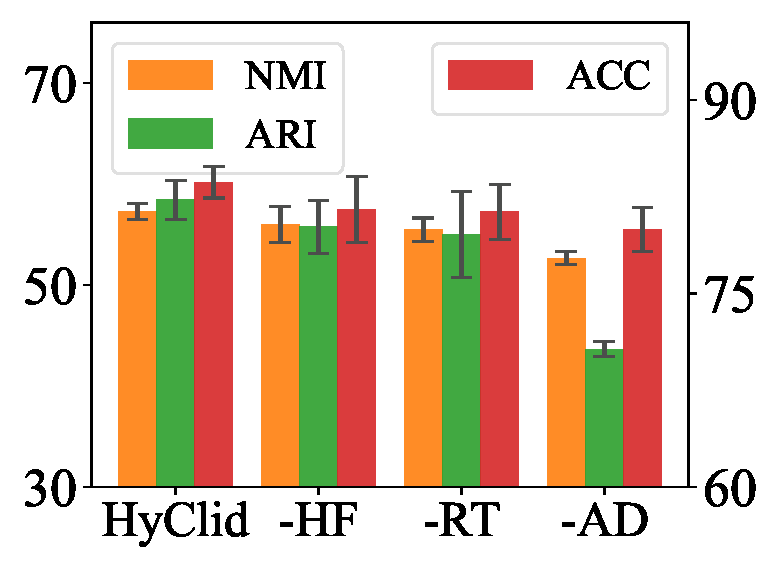
\includegraphics[width=\figwidth\linewidth]{submissions/HyCLID/figures/variant_acm.pdf}}
	%
	\subfigure[][IMDB]{
		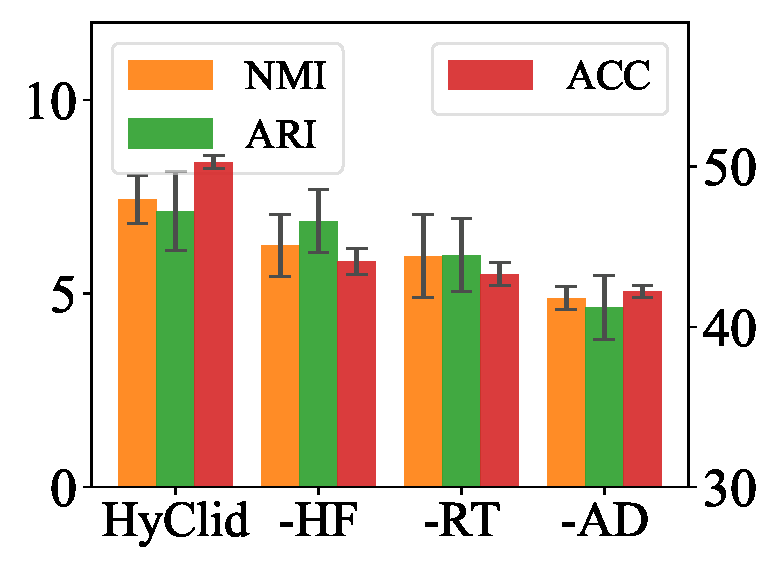
\includegraphics[width=\figwidth\linewidth]{submissions/HyCLID/figures/variant_imdb.pdf}}
	%	
	\subfigure[][MT-S]{
		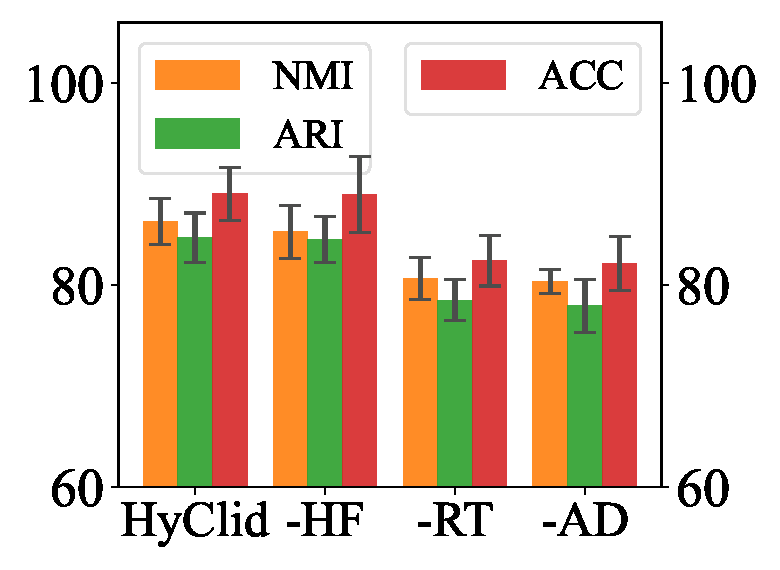
\includegraphics[width=\figwidth\linewidth]{submissions/HyCLID/figures/variant_mtbs.pdf}}
	\caption{Clustering results of different variants. }
	\label{fig:variant}
\end{figure}

As reported in Figure~\ref{fig:variant}, the clustering performance always decreases with the removal of each module. This phenomenon demonstrates the effectiveness of each of the proposed modules.
In detail, compare the best performance achieved by our whole model, \textit{-HF} performs worse, which verifies the existence of the correlations among multiple attributes from the involved objects and conditions and confirms the effectiveness of our rethinking based self-attention to capture these correlations. Next, the fact that \textit{-RT} performs more poorly shows the necessity of our rethinking module for avoiding the omissions of some potential high-orders. Furthermore, when the adaptive mini-batch clustering is further substituted by the traditional clustering assignment hardening~\cite{xie_unsupervised_2016}, \textit{-AD} performs the worst. On the one hand, it shows that problems such as data imbalance make the clustering significantly worse, and on the other hand, it demonstrates that our proposed adaptive module can alleviate this problem very well.


% \subsection{Model Analysis}
\subsection{Case Study for Rethinking Mechanism}
% \vspace{-4pt}
% \subsubsection{Case Study for Rethinking Mechanism}
% \begin{figure}%[!ht]
% 	\centering
% 	\includegraphics[width=0.55\linewidth]{figures/case_study.pdf}
% 	\caption{Heat map visualization for attentive routing-based rethinking mechanism. The rows/columns represent four selected attributes from an interaction case belonging to category ``afternoon tea'' of dataset MT-S, i.e., \textit{lower consumption level}, \textit{student}, \textit{coffee}, \textit{afternoon}, respectively. }
% 	\label{fig:case}
% \end{figure}
\begin{wrapfigure}{r}{0.50\textwidth}
	\centering
	% \vspace{-20pt}
	\includegraphics[width=0.99\linewidth]{submissions/HyCLID/figures/case_study.pdf}
	\caption{Heat map visualization for attentive routing-based rethinking mechanism. The rows/columns represent four selected attributes from an interaction case belonging to category ``afternoon tea'' of dataset MT-S, i.e., \textit{lower consumption level}, \textit{student}, \textit{coffee}, \textit{afternoon}, respectively. }
	\label{fig:case}
	% \vspace{-15pt}
\end{wrapfigure}
In this subsection, we dissect how our attentive routing-based rethinking mechanism works. As shown in Figure~\ref{fig:case}, the heat maps visualize the attention weights of rethinking-based fusion (top) and rethinking-based self-attention (bottom) under two iterations of rethinking (three pairs of heat maps from left to right represent $ r=0, 1, 2 $, respectively).
% The rows/columns represent four selected attributes from an interaction case belonging to category ``afternoon tea'' of dataset MT-S, i.e., \textit{lower consumption level}, \textit{student}, \textit{coffee}, \textit{afternoon}, respectively.



A phenomenon can be observed that, the self-attention assigns relatively high weights to the second-order feature between \textit{coffee} and \textit{afternoon}, while the fusion attention also assigns high weights to \textit{coffee} and \textit{afternoon}. Then, the weights are further growing with the iterations of rethinking. On the contrary, the high weight, assigned to the second-order feature between \textit{lower consumption level} and \textit{afternoon}, is gradually reduced. It validates the effectiveness of our attentive routing-based rethinking mechanism. In detail, it not only encourages the important features or higher-order features through iterative rethinking, but also corrects the overestimated ones.


% \subsubsection{Impact of Number of Propagation Layers}
% \begin{figure}
	\centering
	
	\subfigure[ACM]{
		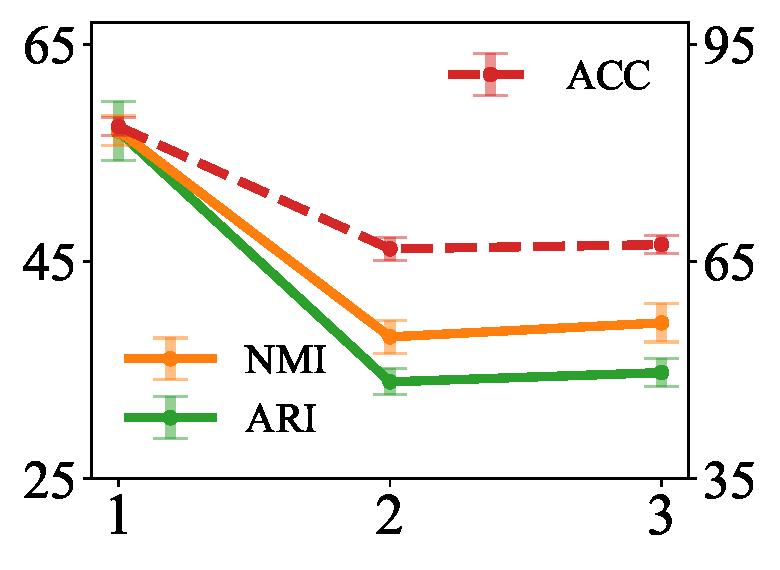
\includegraphics[width=\detailfigwidth\linewidth]{submissions/HyCLID/figures/layer_acm.pdf}}
	%
	\subfigure[IMDB]{
		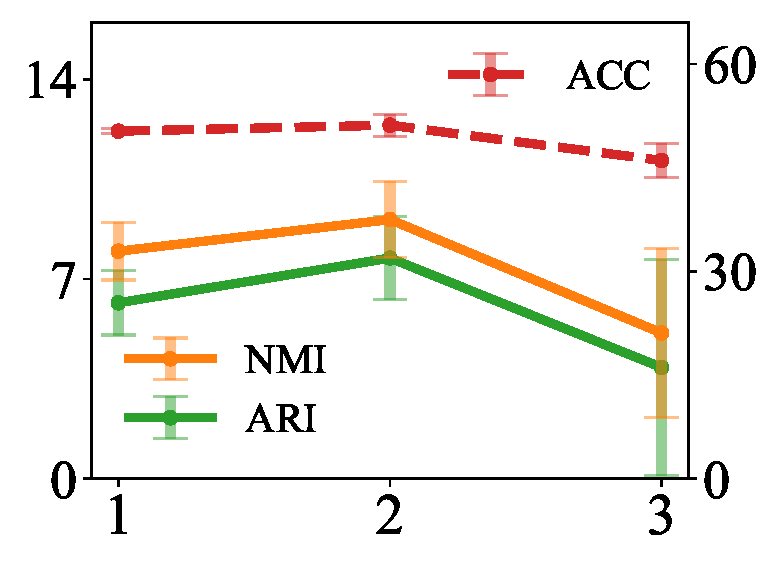
\includegraphics[width=\detailfigwidth\linewidth]{submissions/HyCLID/figures/layer_imdb.pdf}}
	%	
	\subfigure[MT-S]{
		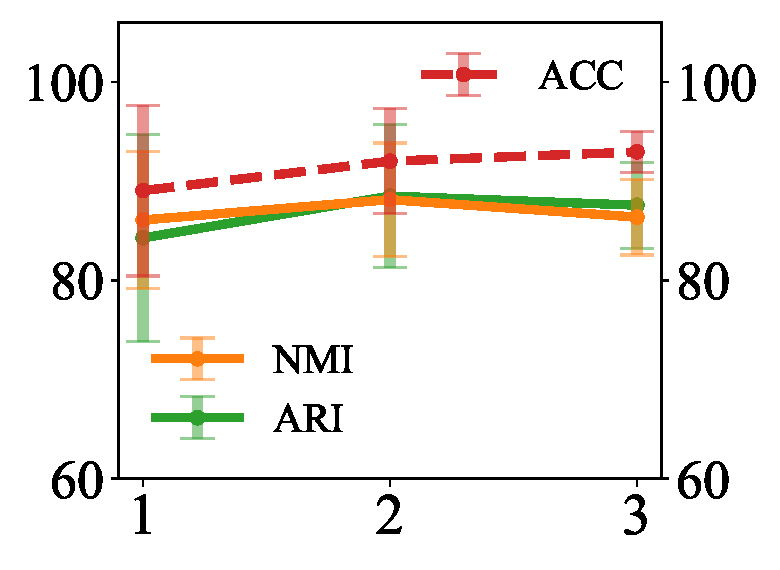
\includegraphics[width=\detailfigwidth\linewidth]{submissions/HyCLID/figures/layer_mtbs.pdf}}
	\caption{Effect of different numbers of propagation layers. }
	\label{fig:layer}
\end{figure}

% In this part, we explore the impact of the number of propagation layers, i.e., the order of neighbors. Specifically, we vary the number of hypergraph propagation layers from 1 to 3. As shown in Figure~\ref{fig:layer}, we have the following observations.

% Specifically, the model could firstly benefit from integrating farther neighbors as more layers are stacked, but then it may be limited by the over smoothing caused by the more increasing depth. Therefore, the best performance occurs when the number of layers is 2 for IMDB and MT-S datasets. On dataset ACM, our \modelname~performs the best when the layer number is 1, and as the number of layers increases, the performance has a noticeable drop. This may be because the connections in ACM are denser and therefore more prone to over-smoothing.


% \subsubsection{Impact of Orders of High-order Feature (Numbers of Self-attention Layers)}
% \begin{figure}
	\centering
	
	\subfigure[ACM]{
		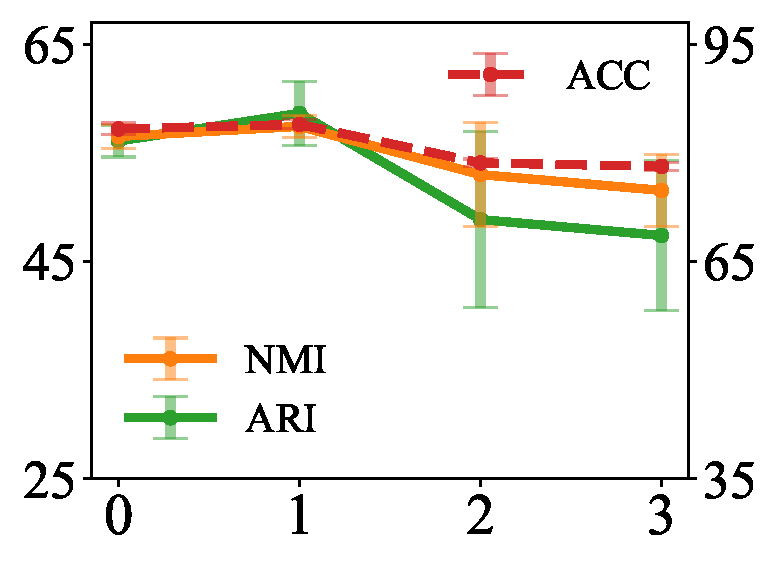
\includegraphics[width=\detailfigwidth\linewidth]{submissions/HyCLID/figures/order_acm.pdf}}
	%
	\subfigure[IMDB]{
		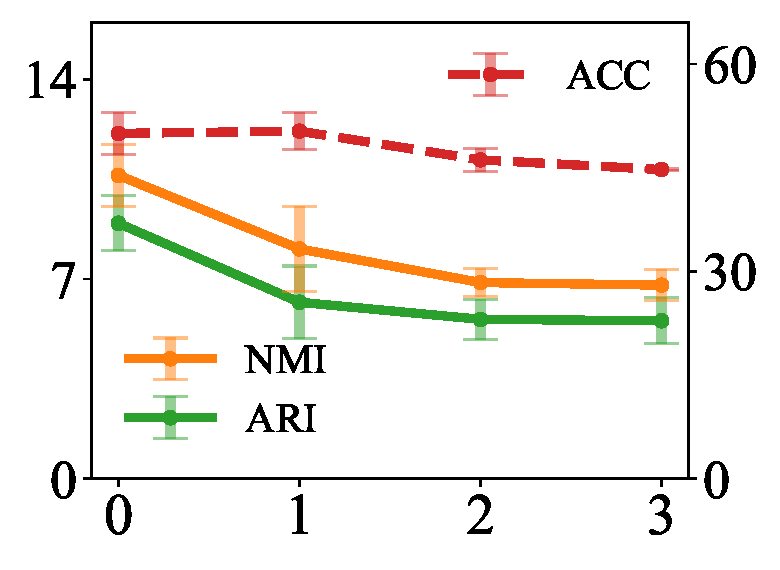
\includegraphics[width=\detailfigwidth\linewidth]{submissions/HyCLID/figures/order_imdb.pdf}}
	%	
	\subfigure[MT-S]{
		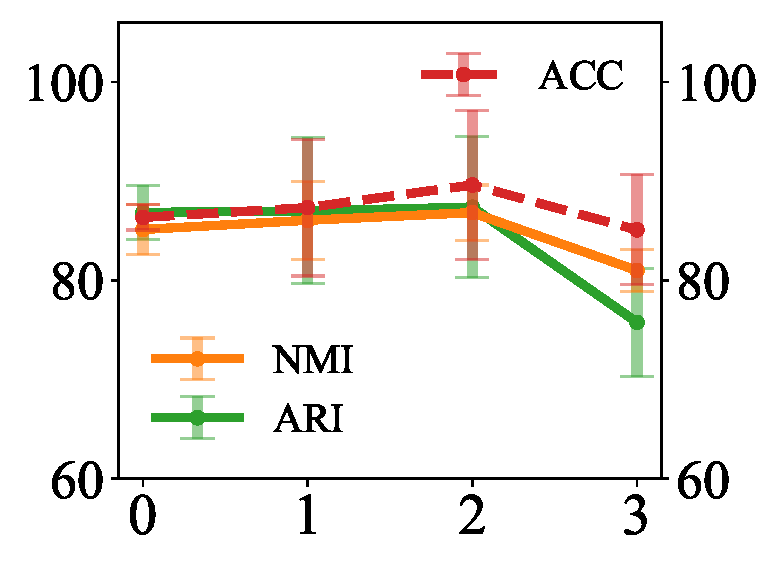
\includegraphics[width=\detailfigwidth\linewidth]{submissions/HyCLID/figures/order_mtbs.pdf}}
	\caption{Effect of different numbers of self-attention layers. }
	\label{fig:order}
\end{figure}

% To investigate the impact of the max orders of high-order features, we vary the number of layers of the rethinking-based self-attention module, while keeping other modules unchanged. Particularly, we report the clustering performance on the three datasets in Figure~\ref{fig:order} with the layer numbers $ p $ in the range of {0, 1, 2, 3}, which represents that the high-order features are of order 1,2,3,4, respectively. The observations are as follows.

% Increasing the max order of features cannot consistently enhance the performance. In detail, on dataset ACM, the clustering performance first increases with the increasing $ p $, and then falls when it is larger than 1. For IMDB, $ p = 0 $ gives the best performance. It means that the high-order features are not required, which in turn increases the training difficulty. Finally, on MT-S, the best performance occurs when $ p = 2 $. It on the one hand shows the desire for the higher-order features by real-world interaction data, and on the other hand verifies the ability of our model to capture high-order features via the proposed rethinking-based self-attention module.


% \subsubsection{Visualization}
% \begin{figure}
	\centering
	
	\subfigure[ACM]{
		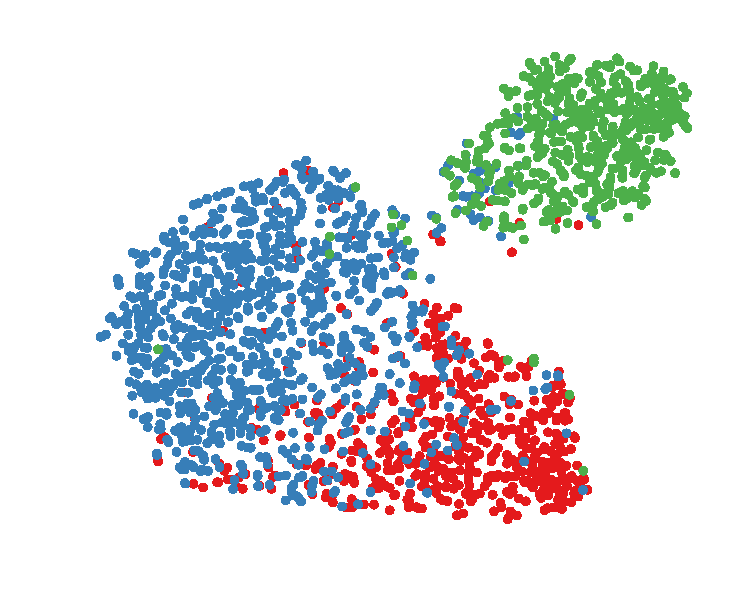
\includegraphics[width=\visualfigwidth\linewidth]{submissions/HyCLID/figures/tsne_acm.pdf}}
	%
	\subfigure[IMDB]{
		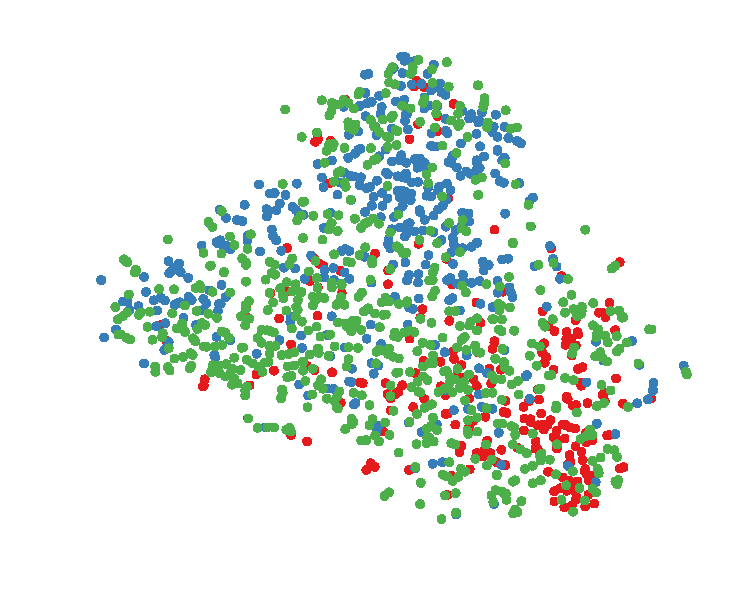
\includegraphics[width=\visualfigwidth\linewidth]{submissions/HyCLID/figures/tsne_imdb.pdf}}
	%	
	\subfigure[MT-S]{
		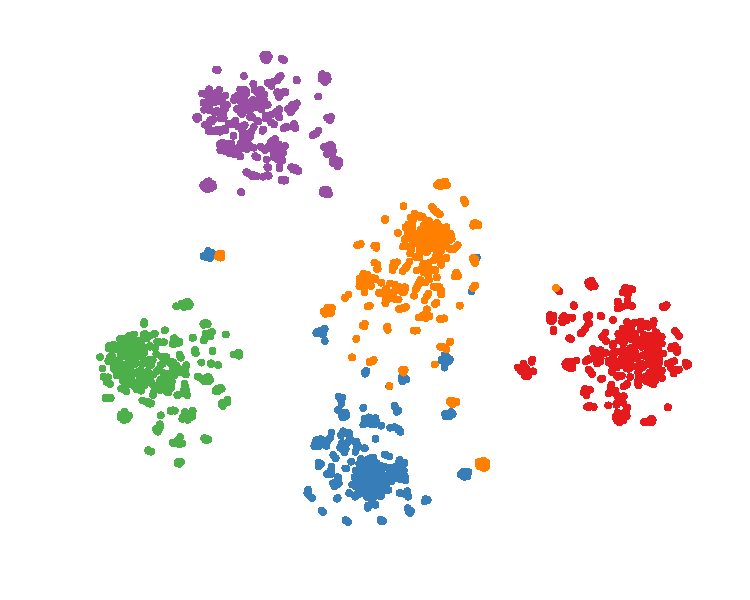
\includegraphics[width=\visualfigwidth\linewidth]{submissions/HyCLID/figures/tsne_mtbs.pdf}}
	\caption{T-SNE visualization of the interaction embeddings. }
	\label{fig:visual}
	\vspace{-4pt}
\end{figure}


% For a more intuitively understanding, in this subsection, we conduct a visualization for the learned interaction embeddings. Specifically, we project the learned interaction embeddings of our \modelname~ into a 2-dimensional space by t-SNE~\cite{van2008visualizing} and visualize them.

% As visualized in Figures~\ref{fig:visual}, an obvious clustering phenomenon can be observed for both ACM and MT-S, while the clustering phenomenon on IMDB is relatively insignificant, which is in line with the scale of NMI and ARI in the previous experiments.


\subsection{Offline Experiment on Recommendation}
% \vspace{-4pt}

In this subsection, we conduct an offline experiment on recommendation to show the applied usage and practical value of our method for food delivery industrial applications, i.e., Meituan Waimai platform. % For convenience,  the experiments are conducted on the large-scale industrial dataset MT-L.
%
Specifically, we divide the MT-L dataset into training/test subsets, i.e., the orders of the first 27 days are for training while those of the last 3 days are for testing. Then we train our model on the training subset of MT-L and then infer the clustering assignments on the test subset. Finally, these learned and inferred clustering assignments are introduced into context-aware recommendation models, e.g., DeepFM~\cite{guo_deepfm_2017} and AutoInt~\cite{song_autoint_2019}, as contexts for CTR prediction, where the dataset partition is the same as above. For comparisons, ``-vanilla'' represents that no clustering assignments are introduced,
%``+TrueTag'' means that the true tags that come with the dataset are used as the context, ``+KMeans'' denotes that the assignments learned by mini-batch KMeans are introduced,
and ``+\modelname'' represents that our \modelname~is adopted for assignments.

% \begin{table}% [!th]
\begin{wraptable}{r}{0.6\linewidth}
\centering
% \vspace{-20pt}
\caption{Top-3 recommendation performance.  }
\resizebox*{0.99\linewidth}{!}{
\begin{tabular}{l|cccccc}
\hline
    Method          & HR            & Recall        & Precision     & NDCG     \\  
\hline 
    DeepFM-vanilla  & 0.5268        & 0.4950        & 0.1849        & 0.4135   \\
%    DeepFM+TrueTag  & 0.5276        & 0.4956        & 0.1859        & 0.4166   \\
%    DeepFM+KMeans   & \ul{0.5290}   & \ul{0.4983}   & \ul{0.1868}   & \ul{0.4185}   \\
    DeepFM+\modelname   & \bf{0.5386}   & \bf{0.5056}   & \bf{0.1868}   & \bf{0.4186}   \\
\hline
    AutoInt-vanilla & 0.5120        & 0.4811        & 0.1786        & 0.4021   \\
%    AutoInt+TrueTag & 0.5154        & 0.4834        & 0.1815        & 0.4050   \\
%    AutoInt+KMeans  & \ul{0.5221}   & \ul{0.4904}   & \ul{0.1842}   & \ul{0.4118}   \\
    AutoInt+\modelname  & \bf{0.5465}   & \bf{0.5142}   & \bf{0.1906}   & \bf{0.4236} \\
% \hline
\hline
\end{tabular}
}
\label{tab:app:rec}
% \vspace{-20pt}
\end{wraptable}
% \end{table}

We report the results on several metrics (including HR, Recall, Precision and NDCG) in Table~\ref{tab:app:rec}. As we can see, for both DeepFM and AutoInt,
%``+TrueTag'' outperforms ``-vanilla'', indicating that the clustering results of interactions are conducive for downstream applications. In addition, the better performance of ``+KMeans'' suggests that more appropriate modeling and stronger learning approaches can discover more accurate patterns of interaction data, which can better help industrial applications. Obviously, ``+\modelname'' achieving the best performance further demonstrates the necessity of our attributed hypergraph modeling of interactions and the effectiveness of our proposed hypergraph clustering network for clustering interactions.
``+\modelname'' outperforms ``-vanilla'', indicating that the clustering results of interactions are conducive for downstream applications and demonstrates the necessity of our attributed hypergraph modeling of interactions and the effectiveness of our proposed hypergraph clustering network for clustering interactions.


\section{Conclusion}
% \vspace{-4pt}
In this paper, we propose a novel clustering task on interaction data to discover more comprehensive cluster patterns, where the interactions are regarded as basic units to be clustered instead of objects.
To this end, we propose a novel Hypergraph CLustering network for Interaction Data, namely \modelname. Specifically, we propose to model the interactions via attributed hypergraph, and then propose a novel rethinking-based hypergraph neural network to learn the representation of interactions. It designs a novel attentive routing-based rethinking mechanism to capture the correlations among multiple attributes of objects and conditions involved in interactions. Besides, we develop an adaptive mini-batch clustering method to deal with the large scale of interaction data, which can further make adaptive adjustments for different data distributions of batches. Extensive experiments verify the effectiveness of our \modelname~on both public datasets and real industrial datasets. Moreover, offline experiments on recommendation show the practical value of our discovered cluster patterns for industrial applications.


%\bibliographystyle{plain}
%\bibliography{submissions/HyCLID/reference}

\begin{thebibliography}{10}

\bibitem{bo_structural_2020}
Deyu Bo, Xiao Wang, Chuan Shi, Meiqi Zhu, Emiao Lu, and Peng Cui.
\newblock Structural {Deep} {Clustering} {Network}.
\newblock In {\em WWW}, 2020.

\bibitem{fan_one2multi_2020}
Shaohua Fan, Xiao Wang, Chuan Shi, Emiao Lu, Ken Lin, and Bai Wang.
\newblock {One2Multi} {Graph} {Autoencoder} for {Multi}-view {Graph}
  {Clustering}.
\newblock In {\em WWW}, pages 3070--3076. ACM, April 2020.

\bibitem{feng_hypergraph_2019}
Yifan Feng, Haoxuan You, Zizhao Zhang, Rongrong Ji, and Yue Gao.
\newblock Hypergraph {Neural} {Networks}.
\newblock In {\em AAAI}, pages 3558--3565, July 2019.

\bibitem{grover_node2vec_2016}
Aditya Grover and Jure Leskovec.
\newblock node2vec: {Scalable} {Feature} {Learning} for {Networks}.
\newblock In {\em {SIGKDD}}, pages 855--864. Association for Computing
  Machinery, 2016.

\bibitem{guo_deepfm_2017}
Huifeng Guo, Ruiming Tang, Yunming Ye, Zhenguo Li, and Xiuqiang He.
\newblock {DeepFM}: {A} {Factorization}-{Machine} {Based} {Neural} {Network}
  for {CTR} {Prediction}.
\newblock In {\em IJCAI}, pages 1725--1731, 2017.

\bibitem{hartigan_algorithm_1979}
J.~A. Hartigan and M.~A. Wong.
\newblock Algorithm {AS} 136: {A} {K}-{Means} {Clustering} {Algorithm}.
\newblock {\em Applied Statistics}, 28(1):100, 1979.

\bibitem{hinton_reducing_2006}
G.~E. Hinton.
\newblock Reducing the {Dimensionality} of {Data} with {Neural} {Networks}.
\newblock {\em Science}, 313(5786):504--507, July 2006.

\bibitem{hu_adaptive_2021}
Youpeng Hu, Xunkai Li, Yujie Wang, Yixuan Wu, Yining Zhao, Chenggang Yan, Jian
  Yin, and Yue Gao.
\newblock Adaptive {Hypergraph} {Auto}-{Encoder} for {Relational} {Data}
  {Clustering}.
\newblock {\em TKDE}, 2021.

\bibitem{hu_heterogeneous_2020}
Ziniu Hu, Yuxiao Dong, Kuansan Wang, and Yizhou Sun.
\newblock Heterogeneous {Graph} {Transformer}.
\newblock In {\em WWW}, pages 2704--2710. ACM, 2020.

\bibitem{kingma_adam_2015}
Diederik~P. Kingma and Jimmy Ba.
\newblock Adam: {A} method for stochastic optimization.
\newblock In {\em ICLR}, 2015.

\bibitem{kipf_variational_2016}
Thomas~N Kipf and Max Welling.
\newblock Variational {Graph} {Auto}-{Encoders}.
\newblock In {\em {NIPS} {Workshop} on {Bayesian} {Deep} {Learning}}, 2016.

\bibitem{kipf_semi_supervised_2017}
Thomas~N. Kipf and Max Welling.
\newblock Semi-{Supervised} {Classification} with {Graph} {Convolutional}
  {Networks}.
\newblock In {\em ICLR}. OpenReview.net, 2017.

\bibitem{kou_social_2016}
Feifei Kou, Junping Du, Yijiang He, and Lingfei Ye.
\newblock Social network search based on semantic analysis and learning.
\newblock {\em CAAI Transactions on Intelligence Technology}, 1(4):293--302,
  October 2016.

\bibitem{li_adaptive_2021}
Xuelong Li, Hongyuan Zhang, and Rui Zhang.
\newblock Adaptive {Graph} {Auto}-{Encoder} for {General} {Data} {Clustering}.
\newblock {\em IEEE Transactions on Pattern Analysis and Machine Intelligence},
  2021.

\bibitem{min_survey_2018}
Erxue Min, Xifeng Guo, Qiang Liu, Gen Zhang, Jianjing Cui, and Jun Long.
\newblock A {Survey} of {Clustering} {With} {Deep} {Learning}: {From} the
  {Perspective} of {Network} {Architecture}.
\newblock {\em IEEE Access}, 6:39501--39514, 2018.

\bibitem{ng2001spectral}
Andrew Ng, Michael Jordan, and Yair Weiss.
\newblock On spectral clustering: Analysis and an algorithm.
\newblock {\em NIPS}, 14, 2001.

\bibitem{shi2018heterogeneous}
Chuan Shi, Binbin Hu, Wayne~Xin Zhao, and S~Yu Philip.
\newblock Heterogeneous information network embedding for recommendation.
\newblock {\em IEEE TKDE}, 31(2):357--370, 2018.

\bibitem{song_deep_2021}
Hanyu Song, Peizhao Li, and Hongfu Liu.
\newblock Deep {Clustering} based {Fair} {Outlier} {Detection}.
\newblock In {\em {SIGKDD} 2021}, June 2021.

\bibitem{song_autoint_2019}
Weiping Song, Chence Shi, Zhiping Xiao, Zhijian Duan, Yewen Xu, Ming Zhang, and
  Jian Tang.
\newblock {AutoInt}: {Automatic} {Feature} {Interaction} {Learning} via
  {Self}-{Attentive} {Neural} {Networks}.
\newblock In {\em CIKM}, pages 1161--1170. ACM, 2019.

\bibitem{tran_directed_2020}
Loc~Hoang Tran and Linh~Hoang Tran.
\newblock Directed hypergraph neural network.
\newblock {\em arXiv}, August 2020.

\bibitem{wang_attributed_2019}
Chun Wang, Shirui Pan, Ruiqi Hu, Guodong Long, Jing Jiang, and Chengqi Zhang.
\newblock Attributed {Graph} {Clustering}: {A} {Deep} {Attentional} {Embedding}
  {Approach}.
\newblock In {\em IJCAI}, August 2019.

\bibitem{wang_heterogeneous_2019}
Xiao Wang, Houye Ji, Chuan Shi, Bai Wang, Yanfang Ye, Peng Cui, and Philip~S.
  Yu.
\newblock Heterogeneous {Graph} {Attention} {Network}.
\newblock In {\em WWW}, 2019.

\bibitem{xie_unsupervised_2016}
Junyuan Xie, Ross Girshick, and Ali Farhadi.
\newblock Unsupervised {Deep} {Embedding} for {Clustering} {Analysis}.
\newblock In {\em ICML}, volume~48, pages 478--487. PMLR, June 2016.

\bibitem{xu_disentangled_2021}
Yichen Xu, Yanqiao Zhu, Feng Yu, Qiang Liu, and Shu Wu.
\newblock Disentangled {Self}-{Attentive} {Neural} {Networks} for
  {Click}-{Through} {Rate} {Prediction}.
\newblock In {\em CIKM}, pages 3553--3557. ACM, 2021.

\bibitem{yadati_hypergcn_2019}
Naganand Yadati, Madhav Nimishakavi, Prateek Yadav, Vikram Nitin, Anand Louis,
  and Partha Talukdar.
\newblock {HyperGCN}: {A} {New} {Method} {For} {Training} {Graph}
  {Convolutional} {Networks} on {Hypergraphs}.
\newblock In {\em NeurIPS}, pages 1511--1522. 2019.

\bibitem{yan_deep_2015}
Yilin Yan, Min Chen, Mei-Ling Shyu, and Shu-Ching Chen.
\newblock Deep {Learning} for {Imbalanced} {Multimedia} {Data}
  {Classification}.
\newblock In {\em {IEEE} {ISM}}, pages 483--488, 2015.

\bibitem{yang2020hypergraph}
Chaoqi Yang, Ruijie Wang, Shuochao Yao, and Tarek Abdelzaher.
\newblock Hypergraph learning with line expansion.
\newblock {\em arXiv preprint arXiv:2005.04843}, 2020.

\bibitem{yang_effective_2021}
Renchi Yang, Jieming Shi, Yin Yang, Keke Huang, Shiqi Zhang, and Xiaokui Xiao.
\newblock Effective and {Scalable} {Clustering} on {Massive} {Attributed}
  {Graphs}.
\newblock In {\em WWW}. ACM, April 2021.

\bibitem{yang_variational_2021}
Shuiqiao Yang, Sunny Verma, Borui Cai, Jiaojiao Jiang, Kun Yu, Fang Chen, and
  Shui Yu.
\newblock Variational {Co}-embedding {Learning} for {Attributed} {Network}
  {Clustering}.
\newblock {\em arXiv}, 2021.

\bibitem{yang_co-clustering_2022}
Tianchi Yang, Cheng Yang, Luhao Zhang, Chuan Shi, Maodi Hu, Huaijun Liu, Tao
  Li, and Dong Wang.
\newblock Co-clustering {Interactions} via {Attentive} {Hypergraph} {Neural}
  {Network}.
\newblock In {\em SIGIR}, pages 859--869. ACM, July 2022.

\bibitem{yun_graph_2019}
Seongjun Yun, Minbyul Jeong, Raehyun Kim, Jaewoo Kang, and Hyunwoo~J Kim.
\newblock Graph {Transformer} {Networks}.
\newblock In {\em NIPS}, volume~32. Curran Associates, Inc., 2019.

\bibitem{zhang_maximum_2021}
Rui Zhang, Hongyuan Zhang, and Xuelong Li.
\newblock Maximum {Joint} {Probability} {With} {Multiple} {Representations} for
  {Clustering}.
\newblock {\em IEEE TNNLS}, pages 1--11, 2021.

\bibitem{zhang_hyper_sagnn_2020}
Ruochi Zhang, Yuesong Zou, and Jian Ma.
\newblock Hyper-{SAGNN}: a self-attention based graph neural network for
  hypergraphs.
\newblock In {\em ICLR}, 2020.

\bibitem{zhou_learning_2006}
Dengyong Zhou, Jiayuan Huang, and Bernhard Schölkopf.
\newblock Learning with {Hypergraphs}: {Clustering}, {Classification}, and
  {Embedding}.
\newblock In {\em NeurIPS}, pages 1601--1608, 2006.

\bibitem{zhu_adaptive_2017}
Xiaofeng Zhu, Yonghua Zhu, Shichao Zhang, Rongyao Hu, and Wei He.
\newblock Adaptive {Hypergraph} {Learning} for {Unsupervised} {Feature}
  {Selection}.
\newblock In {\em IJCAI}, 2017.

\end{thebibliography}

\end{document}

